\documentclass[11pt, a4paper, oneside]{article}

% hifenização e outras especificações para português
\usepackage[portuguese]{babel}

% hiperligações
\usepackage{hyperref}
\hypersetup{colorlinks=true, urlcolor=blue, linkcolor=black}

% escrever acentos e coisas do género sem que o latex se desoriente
\usepackage[utf8]{inputenc}

% para ter imagens, depois define a directoria de imagens
\usepackage{graphicx}
\graphicspath{{./imagens/}}

\usepackage[labelformat=simple]{caption}
\usepackage[labelformat=empty]{subcaption}

% para ter a informação de quantas páginas tem o documento
\usepackage{lastpage}

% definir o cabeçalho e rodapé
\usepackage{fancyhdr}
\pagestyle{fancy}
\fancyhead[L]{\small{Processamento da Wikipédia}}
\fancyhead[R]{\small{Processamento de Linguagens}}

% ter enumerações alinhadas
\usepackage{enumitem}

% escrever algoritmos
\usepackage[algoruled]{algorithm2e}

% mais cores predefinidas
\usepackage[usenames,dvipsnames]{color}

% definir comandos especiais
\newcommand\doubleplus{+\kern-1.3ex+\kern0.8ex} %

\newcommand{\todo}[1] {\textcolor{BrickRed}{\begin{quote}#1\end{quote}}}



%%%%%%%%%%%%%%%%%%%%%%%%%%%%%%%%%%%%%%%%%%%%%%
%% inicio do documento
\begin{document}
\title{Processamento da Wikipédia\\
\begin{normalsize}
Variante 1
\end{normalsize}}
\date{\today\\Universidade do Minho}
\author{
  Bruno Ferreira\\
  {\small A61055}\\
  \and
  Cláudia Oliveira\\
  {\small A60987}\\
  \and
  Vanessa Campos\\
  {\small A54801}\\
}

\maketitle
\begin{abstract}

  O presente trabalho foi desenvolvido no âmbito da Unidade Curricular de Processamento de Linguagens e tem como principal objectivo descrever o processo de desenvolvimento de um analisador léxico da \textit{Wikipédia}. Ao longo deste relatório iremos explicar as estruturas de dados que foram implementadas para o desenvolvimento deste trabalho, bem como todas as decisões que foram tomadas.

\end{abstract}
\newpage

\tableofcontents
\listoffigures 

\newpage
\section{Introdução}

Atualmente a \textit{Wikipédia} é a maior base de dados de conhecimento livre online e disponível em várias línguas, no qual a lingua portuguesa faz parte integrante. Neste contexto, pretende-se desenvolver um Processador de Texto, exportado do \textit{Wikipédia} e gerar a página html com os dados mais relevantes contidos nessa página, utilizando a ferramenta Flex. 
Com este trabalho foi necessário implementar Expressões Regulares de modo a retirar informação mais relevante num contexto enorme de informção, encontrando padrões que nos ajudem a descobrir o tipo de informação que estamos a procura e que é útil no contexto deste caso de estudo.


\newpage
\section{Desenvolvimento}

\subsection{Contextualização do Problema}

Flex é uma ferramenta para gerar automáticamente analisadores léxicos, isto é, programas que reconhecem padrões léxicos num texto. O Flex é uma evolução da ferramenta Lex, mas com a caraterística de ser mais rápido que este (Fast Lex). Lex foi desenvolvido por M.E. Lesk 

\subsubsection{Processamento da \textit{Wikipédia}}

\newpage
\section{WANTED: DEAD OR ALIVE}
\begin{figure}[h!]
  \centering
    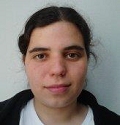
\includegraphics[width=0.6\textwidth]{107}
  \caption[Descrição no titulo]{Descrição abaixo da imagem}
\end{figure}
\newpage

\todo{pode-se utilizar esta tag para chamar a atenção para coisas que é preciso fazer antes de entregar o relatório}

\newpage
\section{Elementos do Grupo}
\begin{figure}[h!]
\centering
\begin{subfigure}{.33\textwidth}
  \centering
  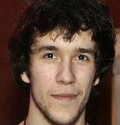
\includegraphics[width=0.8\linewidth]{60}
  \caption{Bruno Ferreira  }
\end{subfigure}%
\begin{subfigure}{.33\textwidth}
  \centering
  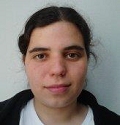
\includegraphics[width=0.8\linewidth]{107}
  \caption{Cláudia Oliveira}
\end{subfigure}%
\begin{subfigure}{.33\textwidth}
  \centering
  
\includegraphics[width=0.8\linewidth]{93}
  \caption{Vanessa Campos}
\end{subfigure}%
\end{figure}


\end{document}